% ------------------------------------------------------------
% Global TikZ styles (textbook-clean defaults)
% ------------------------------------------------------------
\tikzset{
  warp node/.style={circle, draw=black, line width=0.8pt, minimum size=8mm},
  warp edge/.style={->, draw=black, line width=0.6pt},
  warp attach/.style={rectangle, draw=black, dashed, line width=0.5pt, inner sep=3pt},
  warp attachline/.style={dashed, draw=black!70, line width=0.5pt},
  warp note/.style={font=\scriptsize},
  warpstage/.style={rectangle, draw=black, rounded corners=3pt, line width=0.7pt, inner sep=5pt},
  warpartifact/.style={rectangle, draw=black, dashed, rounded corners=3pt, line width=0.5pt, inner sep=4pt},
  warpartifactsmall/.style={rectangle, draw=black, dashed, rounded corners=3pt, line width=0.5pt, inner sep=3pt},
  warpatom/.style={circle, draw=black, fill=black!12, line width=0.5pt, inner sep=1pt, minimum size=5pt},
}

% Reusable TikZ diagrams for the AIΩN Foundations Series
% Requires: \usepackage{tikz} with libraries positioning,calc

\newcommand{\AttachmentSep}{80pt}
\newcommand{\EdgeAttachmentSep}{68pt}

% Diagram A2 — Working example with payload labels
\newcommand{\DiagramCallGraphExample}{
  \begin{tikzpicture}[>=stealth, node distance=5.2cm, every node/.style={font=\small}]
    % Skeleton
    \node[warp node, inner sep=3pt] (vf) {$v_f$};
    \node[warp node, inner sep=3pt, right of=vf] (vg) {$v_g$};
    \draw[warp edge] (vf) -- node[above=10pt] {$e_{\mathrm{call}}$} (vg);
    % Attachments
    \node[warpartifact, rounded corners=4pt, inner sep=5pt, below=\AttachmentSep of vf, xshift=-8pt] (astf) {AST($f$)};
    \node[warpartifact, rounded corners=4pt, inner sep=5pt, below=\AttachmentSep of vg, xshift=8pt] (astg) {AST($g$)};
    \node[warpartifact, rounded corners=6pt, inner sep=6pt, below=\EdgeAttachmentSep of $(vf)!0.5!(vg)$] (prov) {Provenance / profiling};
    \draw[warp attachline] (vf.south) -- ++(0,-10pt) |- (astf.north);
    \draw[warp attachline] (vg.south) -- ++(0,-10pt) |- (astg.north);
    \draw[warp attachline] ($(vf)!0.5!(vg)$) -- ++(0,-10pt) |- (prov.north);
    % Nested WARPs inside attachments (to show recursion)
    \node[warpartifactsmall, below=16pt of astf] (astfsub) {\tiny $\bullet\!\!\!\to\!\!\!\bullet$};
    \draw[warp attachline] (astf.south) -- (astfsub.north);
    \node[warpartifactsmall, below=16pt of astg] (astgsub) {\tiny $\bullet\!\!\!\leftarrow\!\!\!\bullet$};
    \draw[warp attachline] (astg.south) -- (astgsub.north);
    \node[warpartifactsmall, below=16pt of prov] (provsub) {\tiny $\bullet\!-\!\bullet\!-\!\bullet$};
    \draw[warp attachline] (prov.south) -- (provsub.north);
  \end{tikzpicture}}

% Diagram A1b — Tiny WARP: 3 vertices, 2 edges, atom attachments
\newcommand{\DiagramNestedWARP}{
  \begin{tikzpicture}[>=stealth, every node/.style={font=\small}]
    % Outer skeleton (level 2)
    \node[warp node, minimum size=11mm, label=above:{\scriptsize $w_1$}] (w1) {};
    \node[warp node, minimum size=11mm, label=above:{\scriptsize $w_2$}, right=3.2cm of w1] (w2) {};
    \node[warp node, minimum size=11mm, label=above:{\scriptsize $w_3$}, right=3.2cm of w2] (w3) {};
    \draw[warp edge] (w1) -- node[above, warp note] {$e_1$} (w2);
    \draw[warp edge] (w2) -- node[above, warp note] {$e_2$} (w3);

    % Atom attachments on w1, w3
    \node[warpatom, below=1.1cm of w1] (a1) {};
    \node[warpatom, below=1.1cm of w3] (a3) {};
    \draw[warp attachline] (w1) -- (a1);
    \draw[warp attachline] (w3) -- (a3);

    % Atom attachments on edges e1, e2
    \node[warpatom, below=1.0cm of $(w1)!0.5!(w2)$] (ae1) {};
    \node[warpatom, below=1.0cm of $(w2)!0.5!(w3)$] (ae2) {};
    \draw[warp attachline] ($(w1)!0.5!(w2)$) -- (ae1);
    \draw[warp attachline] ($(w2)!0.5!(w3)$) -- (ae2);

    % Nested WARP on w2 (level 1)
    \node[warp node, minimum size=10mm, below=1.4cm of w2, label=above:{\scriptsize $u$}] (u) {};
    \node[warp node, minimum size=10mm, right=2.6cm of u, label=above:{\scriptsize $v$}] (v) {};
    \draw[warp edge] (u) -- node[above, warp note] {$e$} (v);

    % Atom attachments for the nested WARP
    \node[warpatom, below=1.0cm of u] (au) {};
    \node[warpatom, below=1.0cm of v] (av) {};
    \node[warpatom, below=1.0cm of $(u)!0.5!(v)$] (ae) {};
    \draw[warp attachline] (u) -- (au);
    \draw[warp attachline] (v) -- (av);
    \draw[warp attachline] ($(u)!0.5!(v)$) -- (ae);

    % Attachment link indicating w2 hosts the inner WARP
    \draw[warp attachline] (w2.south) -- ++(0,-0.3) |- (u.north);

    % Legend text
    \node[warp note, below=0.35cm of ae] {atoms};
    \node[warp note, above=0.25cm of u] {inner WARP $X_1$};
    \node[warp note, above=0.35cm of w2] {outer skeleton $X_2$};
  \end{tikzpicture}}

% Diagram B — Finite unfolding tower
\newcommand{\DiagramUnfoldingTower}{
  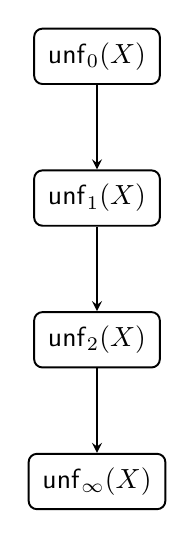
\begin{tikzpicture}[>=stealth, node distance=1.8cm]
    \node (x0) [warpstage] {$\mathsf{unf}_0(X)$};
    \node (x1) [warpstage, below of=x0] {$\mathsf{unf}_1(X)$};
    \node (x2) [warpstage, below of=x1] {$\mathsf{unf}_2(X)$};
    \node (xinfty) [warpstage, below of=x2] {$\mathsf{unf}_\infty(X)$};
    \draw[warp edge] (x0) -- (x1);
    \draw[warp edge] (x1) -- (x2);
    \draw[warp edge] (x2) -- (xinfty);
  \end{tikzpicture}}

% Diagram C — Morphism of WARPs
\newcommand{\DiagramWARPmorphism}{
  \begin{tikzpicture}[>=stealth, node distance=2cm]
    \node[warp node] (Xv1) {$v_1$};
    \node[warp node, right of=Xv1] (Xv2) {$v_2$};
    \draw[warp edge] (Xv1) -- (Xv2);
    \node[warp node, below=2cm of Xv1] (Yv1) {$v'_1$};
    \node[warp node, right of=Yv1] (Yv2) {$v'_2$};
    \draw[warp edge] (Yv1) -- (Yv2);
    \draw[warp edge] (Xv1) -- (Yv1);
    \draw[warp edge] (Xv2) -- (Yv2);
  \end{tikzpicture}}

% Diagram D — Embedding ordinary graph
\newcommand{\DiagramGraphEmbedding}{
  \begin{tikzpicture}[>=stealth, node distance=2.2cm]
    \node[warp node, minimum size=7mm] (a) {$a$};
    \node[warp node, minimum size=7mm, right of=a] (b) {$b$};
    \draw[warp edge] (a) -- node[above] {$e$} (b);
    \node[below=0.8cm of a] (aa) {\footnotesize $\Atom(p_\bullet)$};
    \node[below=0.8cm of b] (bb) {\footnotesize $\Atom(p_\bullet)$};
    \node at ($(a)!0.5!(b)+(0,-1.2)$) {\footnotesize $\Atom(p_\bullet)$ on $e$};
    \draw[warp attachline] (a) -- (aa);
    \draw[warp attachline] (b) -- (bb);
    \draw[warp attachline] ($(a)!0.5!(b)$) -- ($(a)!0.5!(b)+(0,-0.6)$);
  \end{tikzpicture}}
